\section{Evaluation}

\begin{figure}[tb]
	\centering
	%\includegraphics[width=6cm]{}
	\caption{throughput comparison with and without I/O burst buffer}
	\label{throughput}
\end{figure}

\begin{figure}[tb]
	\centering
	%\includegraphics[width=6cm]{}
	\caption{cost comparison with and without I/O burst buffer}
	\label{cost}
\end{figure}

\begin{figure}[tb]
	\centering
	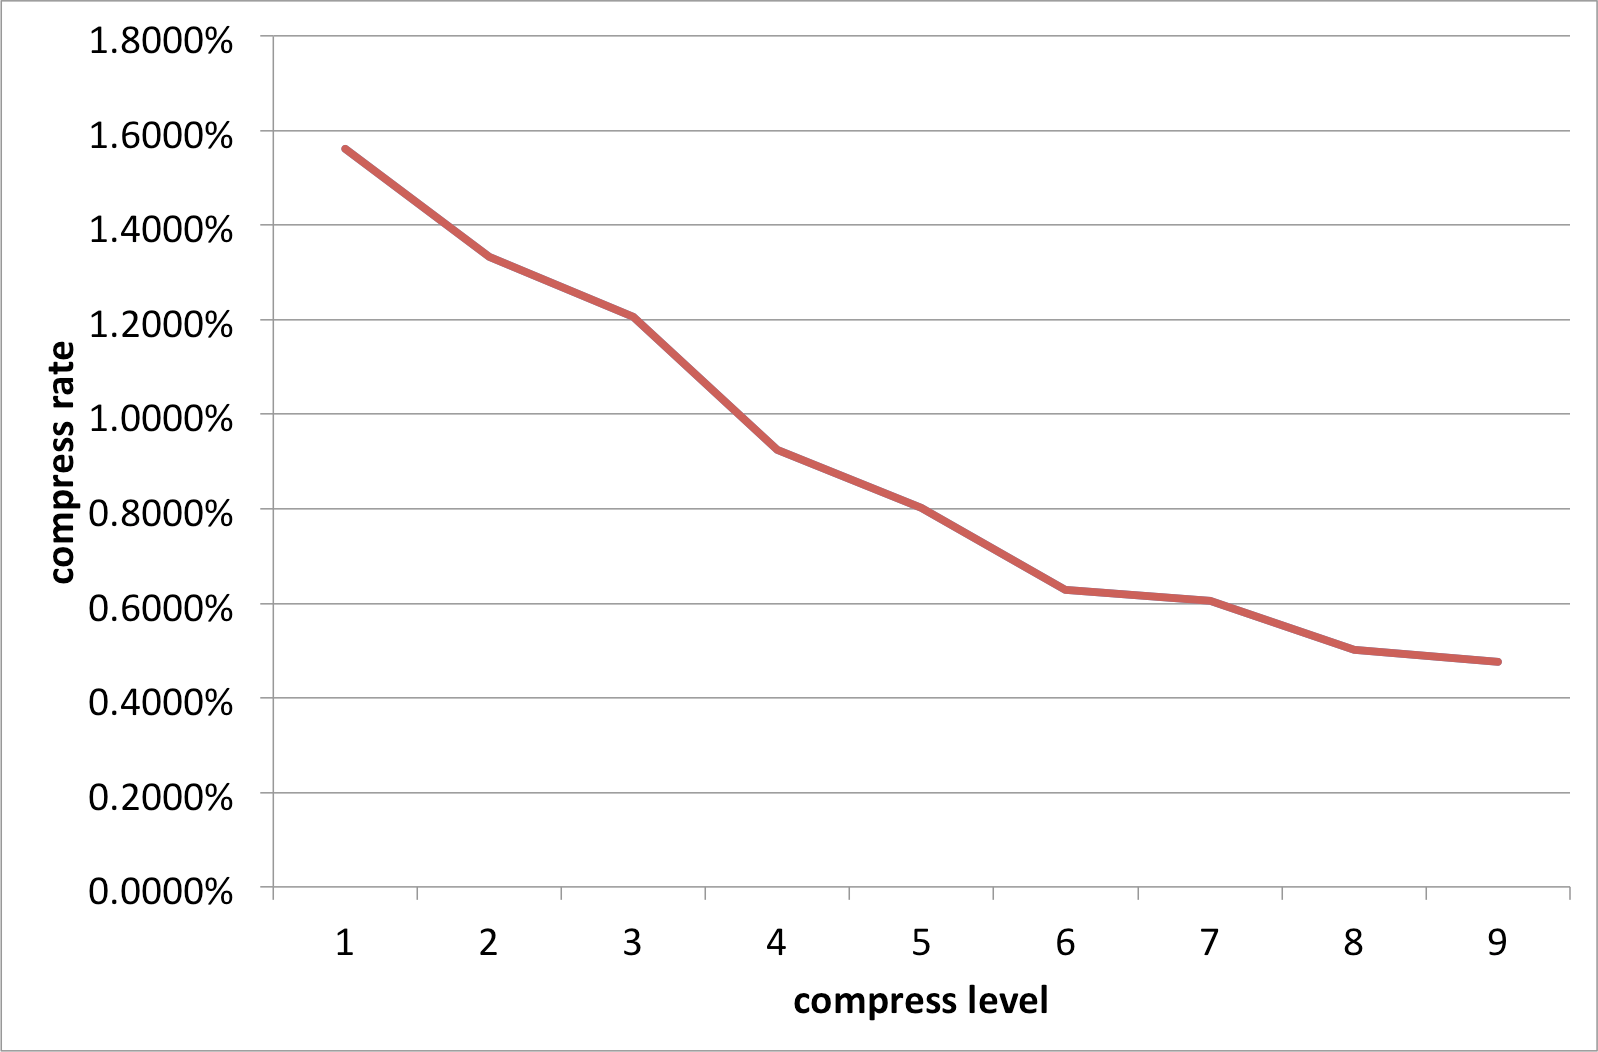
\includegraphics[width=6cm]{compress_rate}
	\caption{compress rate}
	\label{compress rate}
\end{figure}

\begin{figure}[tb]
	\centering
	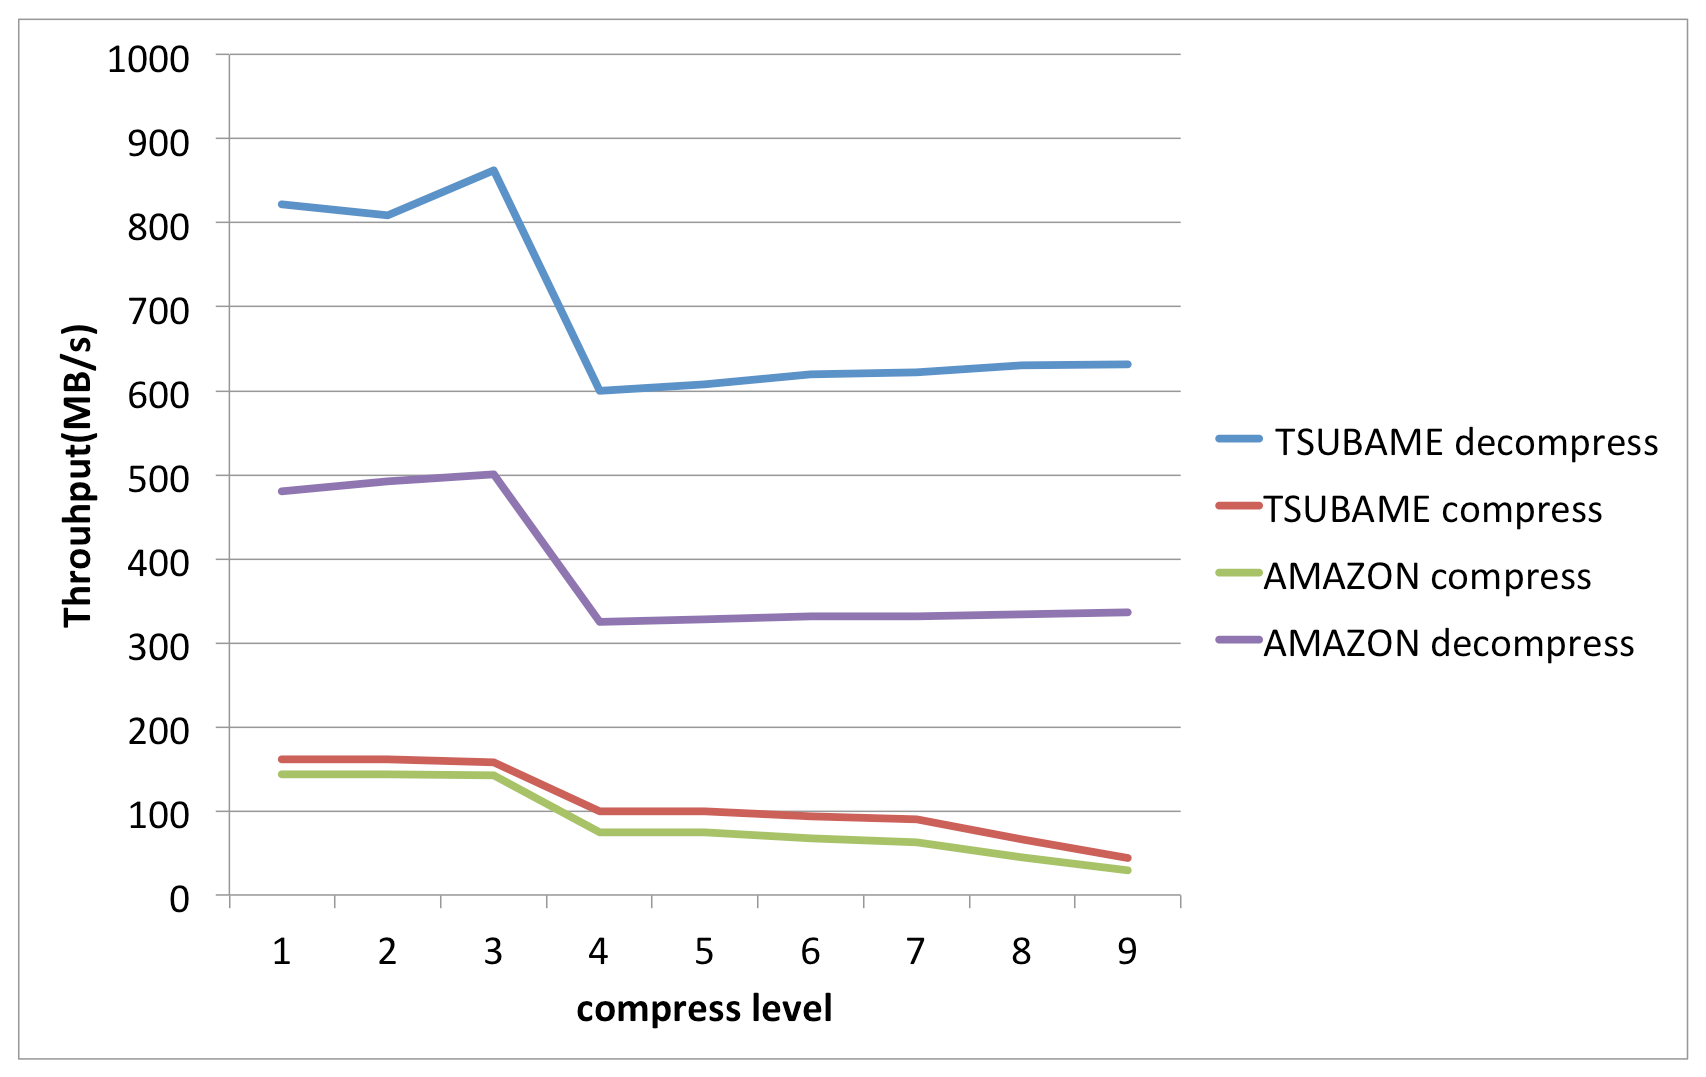
\includegraphics[width=6cm]{compress_time}
	\caption{compress time on TSUBAME V queue and AMAZON EC2}
	\label{compress time}
\end{figure}

\begin{figure}[tb]
	\centering
	%\includegraphics[width=6cm]{}
	\caption{throughput comparison with and without compress}
	\label{compress}
\end{figure}

\begin{figure}[tb]
	\centering
	%\includegraphics
	\caption{cache hit and miss throughput comparison}
	\label{cache hit}
\end{figure}

%\begin{figure}[tb]
%	\centering
%	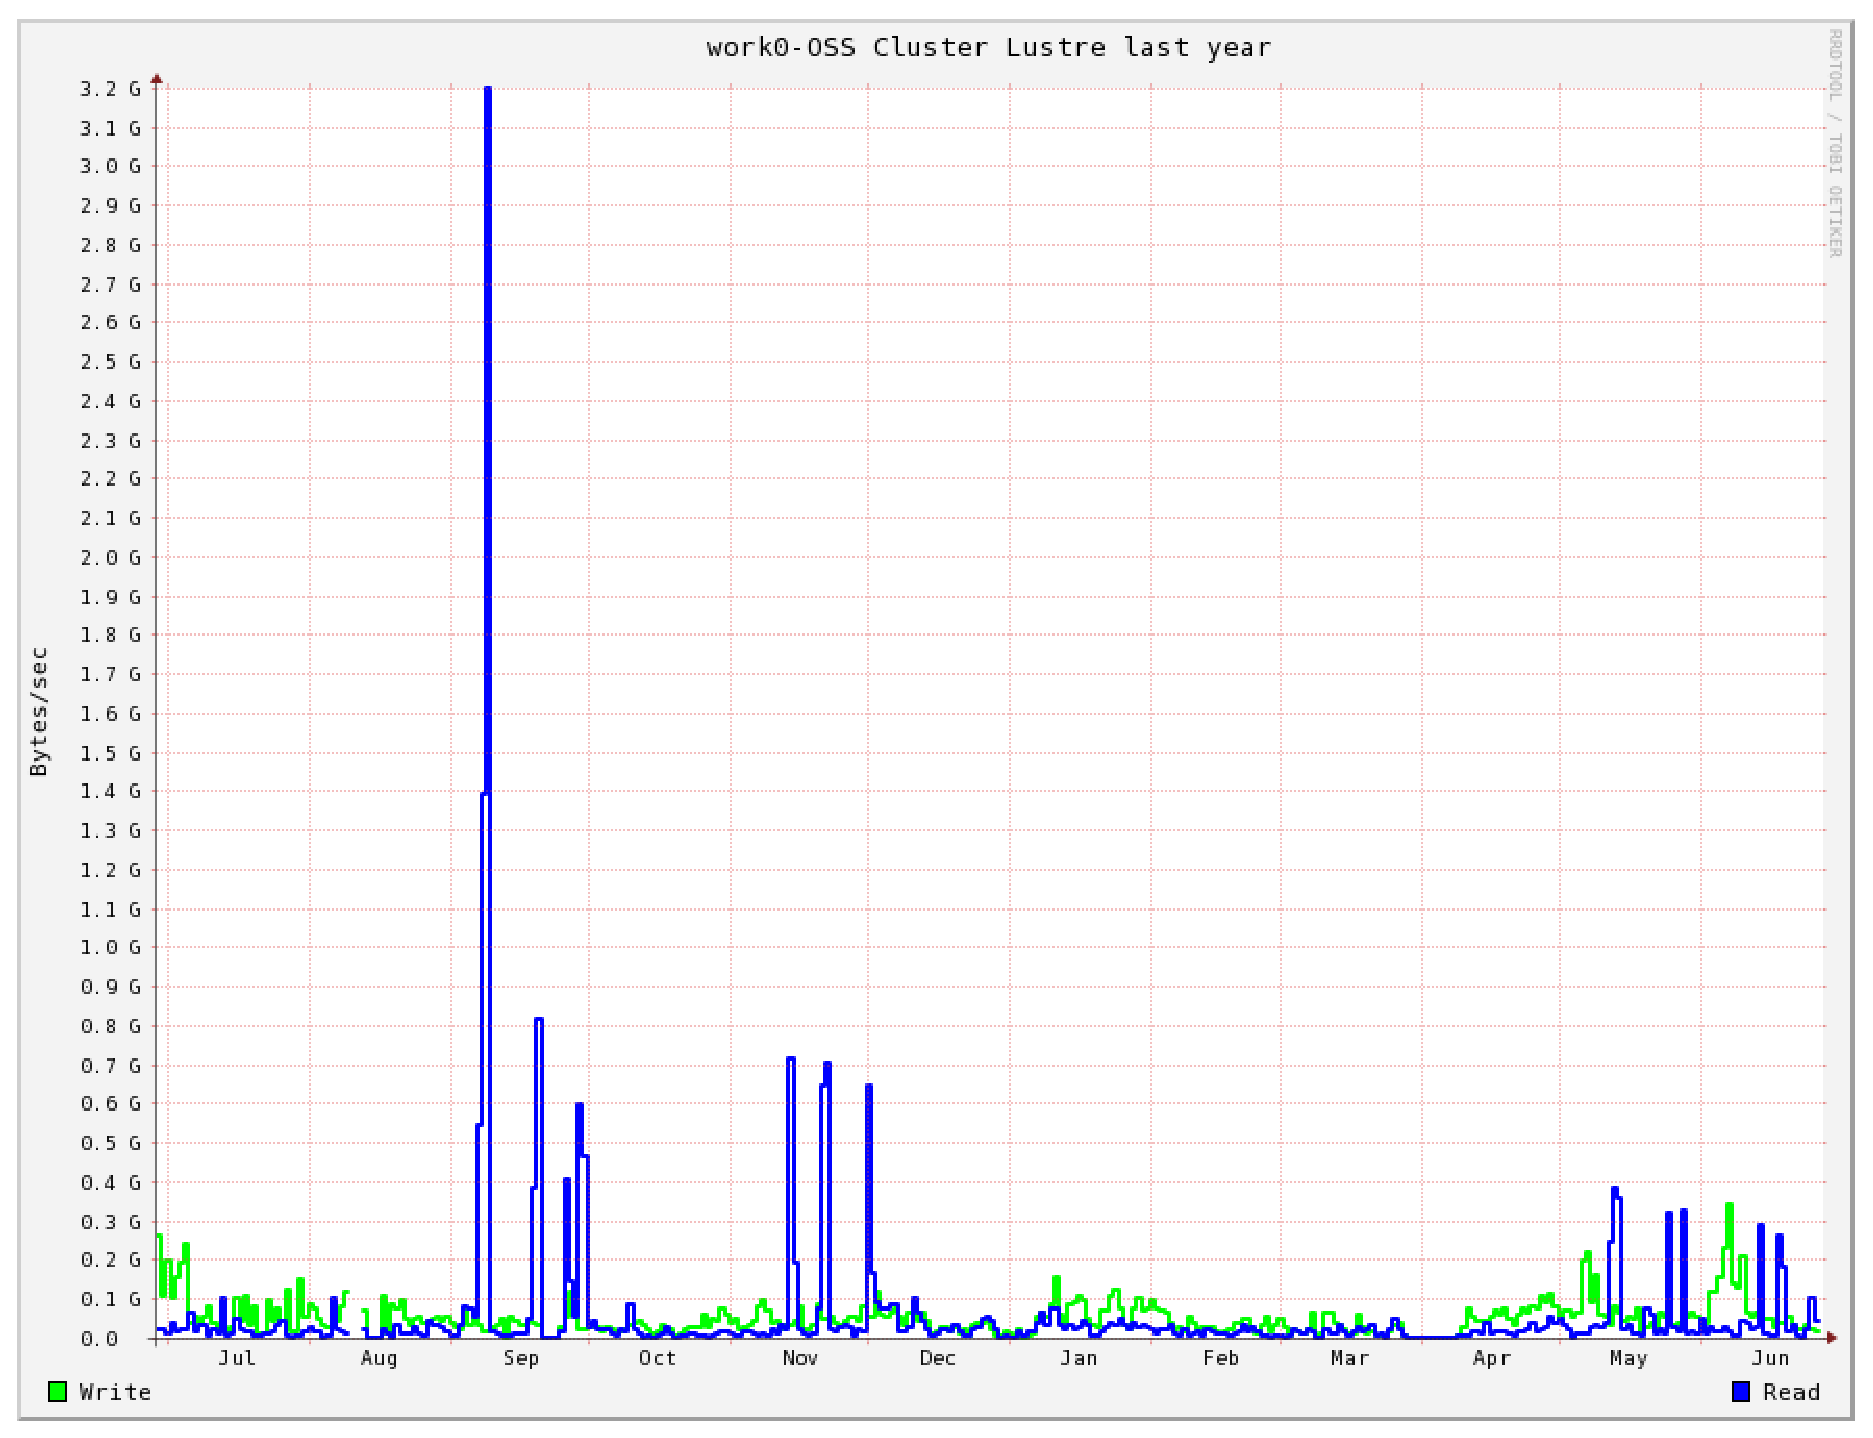
\includegraphics[width=6cm]{tsubamelustre}
%	\caption{TSUBAME Lustre workload}
%	\label{Lustre workload}
%\end{figure}

In this section, a simulation will be introduced based on data taking from several benchmarks on both TSUBAME V queue and AMAZON EC2 public cloud Tokyo region, using
%m3.medium instance, which has a moderate Ethernet condition and one vcpu with 3.75GiB memory, and
m3.xlarge instance, which has a high Ethernet condition and 8 vCPUs with 30GiB memory, run Amazon Linux AMI 2014.03.2(HVM) ( Fig.~\ref{throughput TSUBAME}, Fig.~\ref{throughput AMAZON to OURLAB}. Fig.~\ref{point to point connection AMAZON}, Fig.~\ref{point to point connection LAB} ).
%According to these data and definition described above, we use values defined below.

%\begin{center}
%\begin{tabular}[tb]{|c|c|}\hline
%	$D_2$&$E_1$\\\hline
%	8TB/s&1.08Gbit/s(135MB/s)\\\hline
	
%\end{tabular}
%\end{center}
For throughput between two systems and inside system, from benchmark data, it shows it is hard to achieve a high throughput with only one nodes, and also there is a limit on maximum throughput between two systems and inside system.
Although incresing nodes can increse throughput before reach the maximum, throughput achieved by each nodes decrease because of conflict.
For these reason, we use following formular for throughput between two systems and inside system.
%TSUBAME and AMAZON EC2, we use similar model in \cite{ccgrid}:
\begin{equation}
throughput=-Ax^2+Bx+C~~ A,B>0\\
\end{equation}
we use following equations to determine $A,B,C$
\begin{equation}
\begin{cases}
	-A+B+C=throughput_{one}\\\nonumber
	\frac{B}{2A}=n_{max}\\\nonumber
	-An_{max}^2+Bn_{max}+C=throughput_{max}\\
\end{cases}
\end{equation}

First, we compare throughput with and without I/O buffer nodes.
Since it is hard for one node to fully utilize Internet and Ethernet bandwidth, according to Fig.~\ref{throughput AMAZON to OURLAB}, we assume that one node can achieve half of maximum bandwidth.
We can see from Fig.~\ref{throughput}, when interconnection throughput is larger than Internet throughput, our I/O buffer can achieve a higher throughput.

Then, we compare overall cost by using I/O burst buffer, 

we compare throughput with and without compression, Fig.~\ref{compress rate} shows compress and Fig.~\ref{compress time} shows compress and decompress time on TSUBAME V queue and AMAZON EC2 with a different compress level by using zlib\cite{zlib}.
We can achieve a high compress rate, but the throughput is low, up to 160MB/s, depends on compress level, it is hard to find a compress library can compress data faster and smaller, so the compress throughput may become a bottleneck.
On the other hand, the compress rate is high, since the buffer size is limited, if we can make data smaller, it means we can increase the buffer hit rate, Fig.~\ref{cache hit} shows a throughput comparison between cache miss and hit.

Fig.~\ref{compress}